\documentclass{article}
\usepackage[utf8]{inputenc}

\title{6.172 Homework 8}
\author{Michelle Huang}
\date{November 6, 2017}

\usepackage{amsthm}
\usepackage{amsmath}
\usepackage{amsfonts}
\usepackage[letterpaper, portrait, margin=1in]{geometry}
\usepackage{listings}
\usepackage{graphicx}
\setlength{\parskip}{1em}

\begin{document}
\maketitle
1. Naive approach $n > M/B$: $O(mnr)$ because you have $m$ rows and for each row, you miss all of the accesses to matrix B because a row doesn't fit on a single cache line. Therefore you miss $nr$ for each of the $m$ rows.

Naive approach $M/r < n < M/B$: $M < nr$ and $n < M/B$ means you can fit an entire row into a cache line. The complexity is $O(\frac{mnr}{B})$ because for each row of the first matrix, you get $\frac{nr}{B}$ misses.

Blocking: $O(\frac{mnr}{BM^{0.5}})$ because the number of submatrices is $\frac{mnr}{s^3}$ where $s$ is tuned so that the submatrices fit into the cache ($s = \theta(M^{0.5})$).

Cache Oblivious: This method recursively splits the matrices into 8 different blocks (4 for matrix A, 4 for matrix B). Assuming $m,n,r$ are not too drastically different, we choose to split by $n$ so that our submatrices are still in the right dimension. Thus, we get that our cache misses are the same as that of blocking $O(\frac{mnr}{BM^{0.5}})$. 

2. $2N-1$ space is required because this tableau stores one row and one column at the same time. It only relies on the previous row and previous column to calculate the next row and column. Therefore on each step, it just looks into the table and overwrites the value to store the value of the next row, column data. This takes $2N$ to store the row and column, and the $-1$ comes from the index that is shared between the row and column.

3. 1) $n > M$: This means $n$ is greater than the size of the entire cache. $A(1,1)$ relies on $A(0,0), A(1,0), A(0,1)$. The overall miss rate would be $\frac{n^2}{B}$ because there would be $\frac{n}{B}$ misses for each row and there are $n$ rows. 

2) $n < cM$: There's $\frac{n}{B}$ misses because you miss $\frac{n}{B}$ in the first row and no other misses for the other rows.

4. Work: $\theta(n^2)$ because the total work done is still the same regardless of how you divide it. $T_1(n) = k^2T_1(\frac{n}{k}) + \theta(1)$.
Span: $T_\infty(n) = (2k-1)T_\infty(\frac{n}{k}) + \theta(1)$ because there are $2k-1$ diagonals of the tableau so $T_\infty(n) = \theta(n^{\log_k{2k-1}})$.

5. 1) $Q(n) = \theta(\frac{M}{B})$ if $n < cM$ for sufficiently small constant $c \leq 1$ by submatrix caching lemma, otherwise $4Q(\frac{n}{2}) + \theta(1)$.

2) 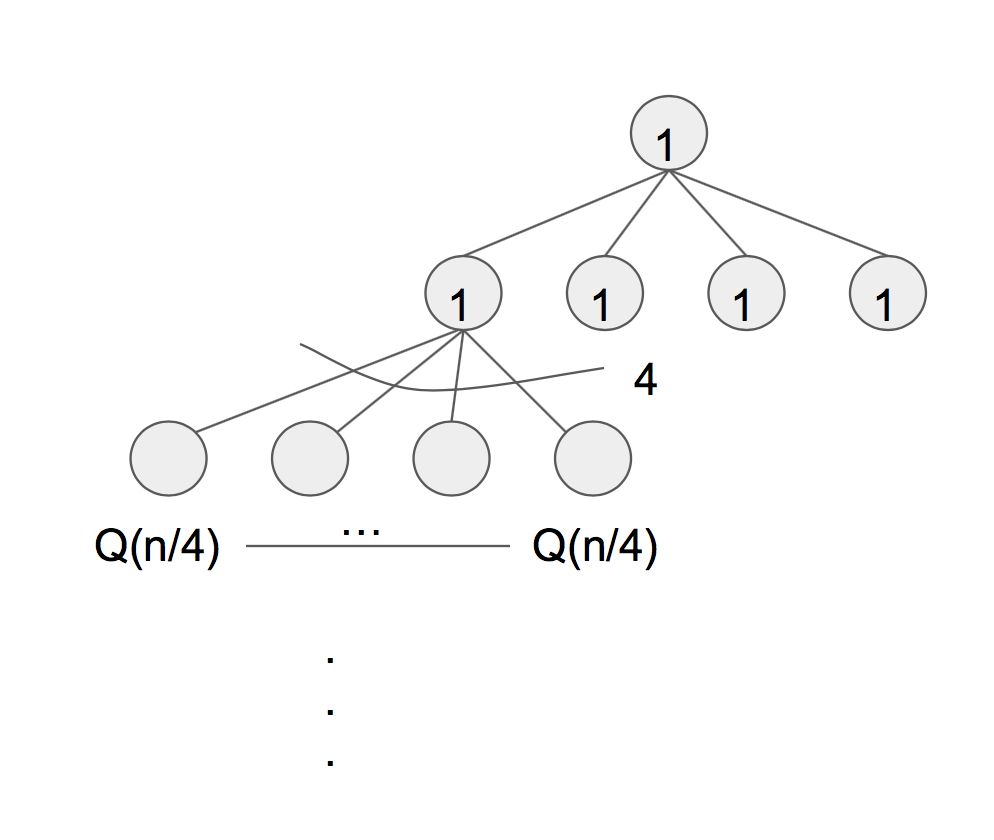
\includegraphics[width=8cm]{tree}

3) Number of leaves is $4^{\lg{n}-\lg{cM}}$

4) $Q(n) = 4^{\lg{n}-\lg{cM}}Q(\frac{n}{2}) + \theta(\frac{M}{B})$

6. If we are unlucky and a subpiece is slightly above cache size, we'd miss on every access so we'd get $\theta(\frac{n^2}{MB})$ misses for all of the $k$ rows, resulting in $\theta(\frac{n^2k}{MB})$ misses total. However, if we are lucky and every subpiece fits, then we'd only miss on the initial $\theta(\frac{n^2}{MB})$ and not incur a miss for each of the $k$ rows.


\end{document}

